\documentclass{article}
\usepackage{multirow}
\usepackage{float}
\usepackage{fancyvrb}
\usepackage{graphicx}

\title{\vspace{-2.0cm}BIOINF 704 Assignment 2}

\author{Badi James (bjam575)}

\begin{document}
	
	\maketitle
	
	\section{Accuracy of parameter estimation for logistic model of association:}
	
	\paragraph{}The logistic model is a way of modelling the association between two alleles (ie $A$ and $a$) at a locus and a binary phenotype (i.e trait that is either absent or present). It is described as follows: \\
	$p_g =$ probability that an individual of genotype $g$ has the trait. $g \in \{0,1,2\}$ assigned to genotypes $AA$, $Aa$ and $aa$ respectively. \\
	Log odds for $g$: \[= \log(\frac{p_g}{1 - p_g}) = \beta_0 + g \beta_1\]
	$\beta_0$ and $\beta_1$ are parameters that have to be estimated. The log likelihood of a given pair of values for these parameters can be calculated given a data set of genotype-phenotype pairs for each individual. First the above log odds equation is solved for each $p_g$. Second, the log likelihoods for each individual in the data having their phenotype given their genotype are calculated. Then these log likelihoods are summed together to get the log likelihood of the parameter values. With this a maximum likelihood (ML) approach can be taken when estimating values for $\beta_0$ and $\beta_1$.
	
	\paragraph{} However it is important to assess the accuracy of the parameter estimates. Estimating the variance of the parameters is a way of investigating this. This assignment demonstrates the non parametric bootstrap technique as a method of estimating variance.
	
	Using this data set $D$ of size $N = 31$:
	\begin{verbatim}
	phenotype:	1 1 1 1 1 1 1 1 1 1 1 1 1 1 1 1 1 1 1 0 0 0 0 0 0 0 0 0 0 0 0
	genotype:  0 0 0 0 0 0 0 0 0 0 1 1 1 2 2 2 2 2 2 0 0 0 0 0 0 1 1 1 1 1 2
	\end{verbatim}	
	$B = 100$ bootstap samples each of size $N$ were created by sampling with replacement from $D$. For each bootstrap sample, maximum likelihood estimates of $\beta_0$ and $\beta_1$ were found. This was done using the optim function in R, set to maximize instead of minimize, with starting values of $\beta_0 = 0.1$ and $\beta_1 = 0.2$. Otherwise default parameters for optim were used, meaning that the Nelder and Mead (1965) method was used to find the ML estimates. Then the variance of each $\beta$ was estimated using the formula:
	\[\hat{var}(\beta) = \frac{\sum^{B}_{b=1}(\beta_b - \bar{\beta})^2}{B - 1}\] 
	where $\beta_b$ is the estimate for the parameter for bootstrap sample $b$ and $\bar{\beta}$ is the mean estimate for the parameter across all bootstrap samples.
	
	\paragraph{}The results are:
	\[\hat{var}(\beta_0) = 0.1926\]
	\[\hat{var}(\beta_1) = 0.1715\]
	\[\bar{\beta_0} = 0.2260\]
	\[\bar{\beta_1} = 0.3533\]
	
	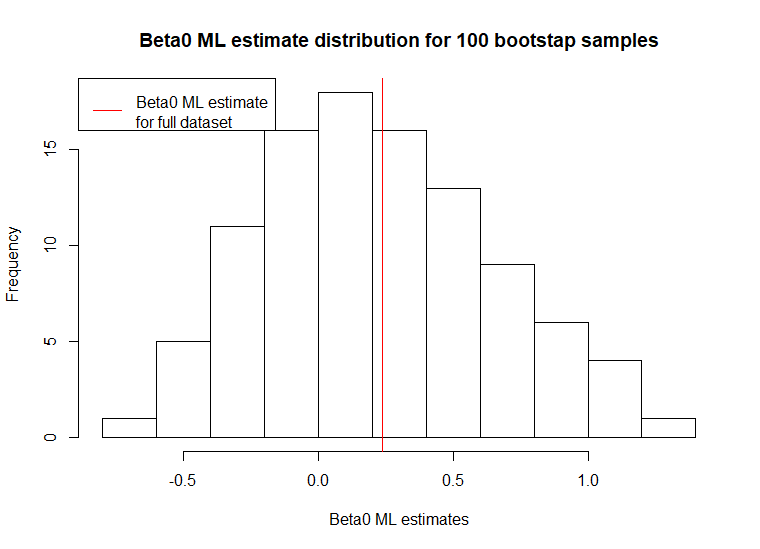
\includegraphics[scale=0.53]{Beta0}\\
	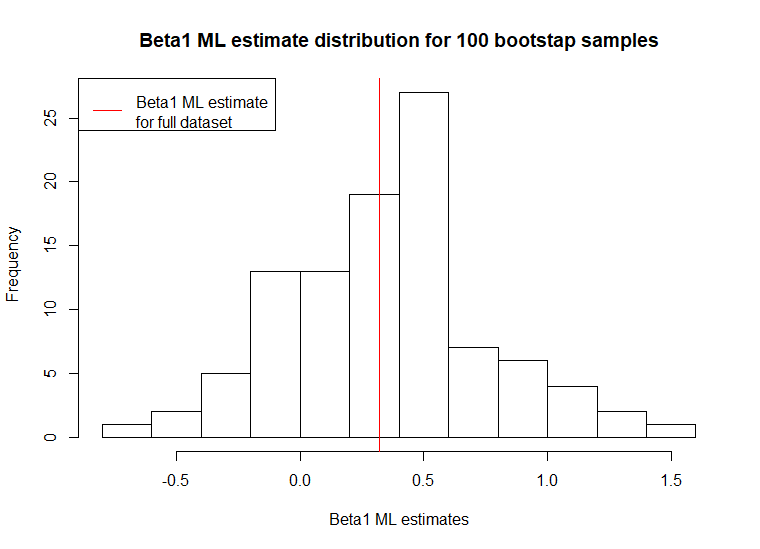
\includegraphics[scale=0.53]{Beta1}\\
	
	\paragraph{} 
	
	
\end{document}